%\documentclass{tnreport}
%\documentclass[stage1a]{tnreport} % If you are in 1nd year
\documentclass[stage2a]{tnreport} % If you are in 2nd year
%\documentclass[confidential]{tnreport} % If you are writing confidential report
%\documentclass[english]{tnreport} % If you are writing your report in english

\newcommand{\comment}[1]{}

\usepackage{url}
\usepackage{float}


\def\reportTitle{Développement d'un chatbot pour Mattermost via les technologies de Google Cloud} % Titre du mémoire
%\def\reportLongTitle{Winter is Coming -- You know nothing Jon Snow} % Titre plus long du mémoire

\def\reportAuthor{Malaury Keslick}
\def\reportAuthorEmail{\email{malaury.keslick@telecomnancy.eu}} % Courriel de l'élève

% This is an example, for a report with several students as authors
%\def\reportAuthor{Jon Snow\\ Samwell Tarly}
%\def\reportAuthorEmail{\email{jon@castleblack.com}\\ \email{tarly@casteblack.com}} % Courriel de l'élève

\def\reportAuthorAddress{18 Boulevard du Maréchal Foch} % Adresse de l'élève
\def\reportAuthorCity{54520, Laxou} % Adresse (cont.) de l'élève
\def\reportAuthorPhone{+33 (0)6 02 22 43 53} % Téléphone de l'élève

%\def\reportIndustrialSupervisor{Eddard Stark} % Prénom Nom de l'encadrant industriel
\def\reportSupervisor{François Charoy} % Prénom Nom de l'encadrant industriel (en entreprise ou laboratoire)
\def\reportAcademicSupervisor{Gérald Oster} % Prénom Nom de l'encadrant académique

% For PIDR ?
%\def\reportSupervisor{Eddard Stark} % Prénom Nom de l'encadrant industriel
%\def\reportProjectCustomer{Projet réalisé pour l'équipe Night's Watch du laboratoire HBO}

\def\reportCompany{Inria Nancy Grand-Est} % Nom de l'entreprise d'accueil
\def\reportCompanyAddress{615 Rue du Jardin Botanique}  % Adresse de l'entreprise
\def\reportCompanyCity{54600 Villers-lès-Nancy} % Adresse (cont.) de l'entreprise
\def\reportCompanyPhone{+33 (0)3 83 59 30 00} % Téléphone de l'entreprise
\def\reportCompanyLogoPath{figures/logo_inria} % Logo de l'entreprise -- comment this definition to remove company logo

\def\place{Laxou} % Ville pour la signature pour l'engagement anti-plagiat
\def\date{\today} % Date pour la signature de l'engagement anti-plagiat

\makeatletter
\g@addto@macro{\UrlBreaks}{\UrlOrds}
\makeatother

\begin{document}

\maketitle
\pagenumbering{roman}

\insertAntiPlagiarismAgreement{Keslick, Malaury}{31814820}

% You may insert several agreement in case of multiple authors
%\insertAntiPlagiarismAgreement{Tarly, Samwell}{2014031142}

\clearpage

\makesecondtitle

\section*{Remerciements}
\addcontentsline{toc}{chapter}{Remerciements}

{\em
Tout d'abord je souhaiterai remercier mon maître de stage, Monsieur François Charoy, qui m'a offert une belle opportunité de poursuivre ma découverte du monde de la recherche malgré la situation de crise que traverse notre pays. Merci à lui d'avoir apporté sa bonne humeur de façon lors de nos réunions hebdomadaires en visio-conférence, elles m'auront permis de garder un rythme essentiel à ma réussite de ce stage. \\

Je tiens également à remercier tout particulièrement Madame Clélie Amiot pour son suivi inégalable et son accueil si chaleureux. \\

Un grand merci à toute l'équipe Coast du Loria, que j'ai pu rencontrer à travers mon écran et lors notre pique-nique, pour sa joie de vivre et nos échanges toujours intéressants. \\

Enfin, je souhaite adresser mes remerciements à toute l'équipe pédagogique et administrative de TELECOM Nancy pour avoir permis la réalisation de ce stage.
}



\clearpage

\renewcommand{\baselinestretch}{0.5}\normalsize
\tableofcontents
\renewcommand{\baselinestretch}{1.0}\normalsize
\cleardoublepage

\pagenumbering{arabic}
\setcounter{page}{1}

\chapter{Introduction}

Les outils de communication en ligne sont de nos jours de plus en plus présents, qu'ils soient à usage personnel ou professionnel. C'est dans ce cadre qu'on été introduit les premiers chatbots dans les années 1960. Assistants virtuels répondant automatiquement aux messages d'un ou de plusieurs utilisateurs, ils étaient à leur création très primaires, et ne pouvaient répondre qu'à un faible nombre de messages mais ils sont aujourd'hui toujours plus performant et sont utilisés dans pratiquement tous les domaines, allant de la modération de messages à l'assistance à un client souhaitant réserver son billet de train. \\

C'est dans le cadre d'une étude sur les collaborations entre systèmes informatiques et utilisateurs que s'inscrit le projet d'évaluation de la confiance dans la collaboration entre les chatbots et les humains sur lequel j'ai travaillé lors de ces neuf semaines de stage au sein de l'équipe Coast du Loria. Ce stage s'inscrit dans mon cursus d'élève ingénieur au sein de TELECOM Nancy, se déroulant au terme de ma deuxième année durant laquelle je me suis spécialisée en \textbf{I}ngénierie \textbf{L}ogicielle. Ayant déjà travaillé au sein de cette équipe de projet lors de mon PIDR, j'ai eu la chance de pouvoir découvrir un autre aspect de ce domaine de recherche lors de ces quelques semaines. \\

Tout d'abord j'effectuerai une présentation du centre de recherches, puis je présenterai la problématique de mon stage en introduisant la notion de chatbot et en explicitant le projet que l'on m'a confié lors de ce stage, à savoir le développement d'un agent conversationnel à l'aide des outils Google Cloud. Je détaillerai ensuite leur réalisation et validation avant de dresser le bilan de ce stage et de finalement conclure.\\



\clearpage

\chapter{Présentation du centre de recherches}

%à retravailler%

L'INRIA (\textbf{I}nstitut \textbf{N}ational de \textbf{R}echerche en \textbf{I}nformatique et \textbf{A}utomatique) est un établissement français public de recherche en sciences et technologies du numérique.  Il a été fondé en 1967 et est affilié au Ministère de \emph{l'Education Nationale, de l'Enseignement supérieur et de la Recherche}. Jusqu'en 2008, son activité est centralisée dans son siège social à Rocquencourt, puis sont ensuite créés huit centres de cherche indépendants dans toute la France : ceux de Bordeaux, Grenoble, Lille, Nancy, Paris, Rennes, Palaiseau et Biot. Un premier centre hors de la France a également été inauguré en 2012, au Chili. Ces 9 pôles de recherche rassemblent plus de 3500 scientifiques travaillant au sein de plus de 200 équipes-projets en partenariat avec de grandes universités de recherche et des partenaires industriels. En 2018, tous ces ambitieux projets ont été soutenus d'un budget de 236 millions d'euros. \\

Chaque centre de recherche a ses propres positionnements et enjeux stratégiques. Nous allons nous concentrer sur le cas du centre Nancy - Grand Est, puisqu'il est celui où j'ai réalisé mon stage. Sous la direction de Bruno Lévy, ce centre rassemble plus de 400 scientifiques issus de 45 nationalités différentes, au service de la recherche et de l'innovation. Ses axes scientifiques prioritaires sont l'intelligence algorithmique et les interactions Hardware-Software. De plus, le centre est en étroit lien avec l'Université de Lorraine pour une excellente dynamique de site, et un travail est fait sur le développement de l'antenne sur le site de Strasbourg (qui sera axée sur la médecine personnalisée), avec de nouveaux partenariats stratégiques et une possibilité accrue de coopérations transfrontalières avec l'Allemagne. \\
Le siège Nancy - Grand Est compte un grand nombre de partenaires, qu'ils soient académiques (universités de Lorraine et Strasbourg, iCube, CNRS, institut Max-Planck pour l'informatique de Sarrebruck) ou entrepreunariaux allant des Startups aux grands groupes comme Orange, Thales ou encore Facebook. \\

Les 22 équipes de Nancy travaillent sur des thèmes divers et variés allant de la génétique à la cryptologie. Lors de mon stage, j'ai intégré l'équipe \emph{COAST}, composée d'une petite trentaine de personnes (enseignants-chercheurs, doctorants, ingénieurs, stagiaires). Dirigée par François Charoy, cette équipe travaille sur les systèmes collaboratifs, la gestion des processus métiers, la réplication optimiste et l'informatique orientée service. Les axes de recherche de l'équipe sont alors les suivants ~\cite{COAST}: 
\begin{itemize}
    \item  La gestion sure et efficace de données collaboratives à large échelle en terme de quantité de données et d’utilisateurs de ces données ;
    \item La composition de services orientés données pour permettre la construction d’applications à l’échelle du Web et pour donner des garanties sur le fonctionnement de ces applications ;
    \item Le support à la construction d’environnements collaboratifs pour lesquels on puisse déterminer un niveau de confiance et de sécurité (axe sur lequel mon stage était dirigé).
\end{itemize}

\clearpage

\chapter{Problématique}

Lors de mon stage, j'ai eu a développer un robot conversationnel dans un outil permettant de gérer les échanges entre utilisateurs, Mattermost. Cette application est une plateforme permettant de créer des équipes de personnes afin qu'elles puissent converser entre elles de manière organisée. Dans une équipe, on peut aller créer différents canaux qui permettront de bien distinguer chaque espace de travail. De plus, on peut également attribuer un certain niveau de confidentialité à un canal (accessible à tous les membres ou alors uniquement sur invitation), et envoyer des messages privés à chaque utilisateur de son équipe (voir fig. \ref{MM}). Ce bot a pour but d'être capable de retrouver dans une conversation ou dans un canal des informations données par un utilisateur pour les transmettre à un autre utilisateur en fonction des demandes. Ce bot devait être implémenté via les fonctionnalité d'un cloud, pour ma part celui de Google, tandis que mon co-équiper Frédéric Vaz effectuait le même travail en utilisant les services de Microsoft Azure. \\

Dans cette partie je vous présenterai d'abord ce que sont les chatbots avant de préciser la problématique sur laquelle mon travail a porté. \\


\section{Les chatbots}

Dans un premier temps, je vais vous présenter ce qu'est un chatbot, et quelles peuvent être ses utilités. Francisé comme ``agent conversationnel'', un chatbot est un programme informatique capable de simuler un échange avec un ou plusieurs partis, que ce soit par échange vocal ou textuel. Ils sont aujourd'hui utilisés à de nombreux niveaux, que ce soit pour faciliter la communication inter-entreprise, ou pour rendre un service à des clients, comme le montre l'image suivante [fig. \ref{chatbot}]. \\

\begin{figure}[h!]
    \centering
    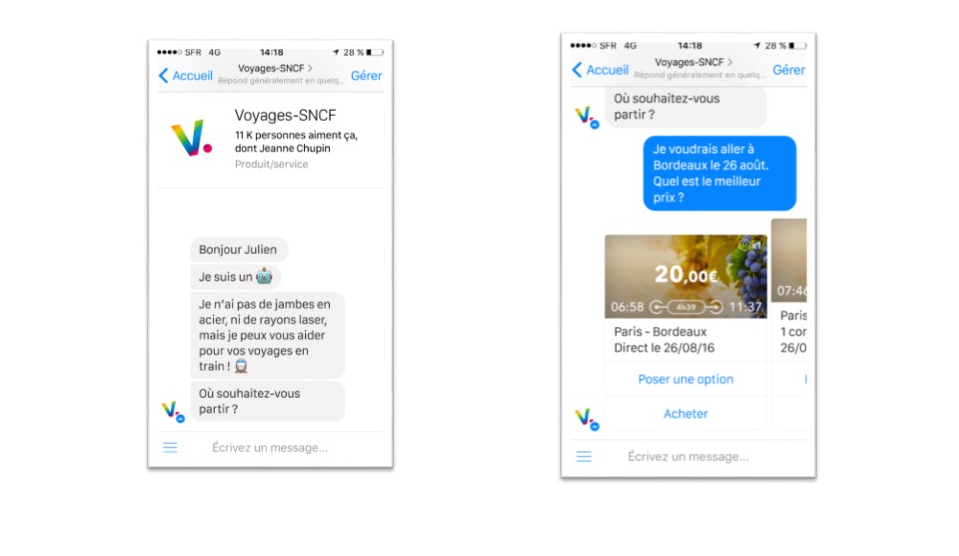
\includegraphics[width=0.7\textwidth]{figures/bot_sncf.png}
    \caption{Exemple d'un chatbot de la SNCF destiné à la clientèle~\cite{BotSNCF}}
    \label{chatbot}
\end{figure}


\vspace{\linewidth}
Le premier chatbot, nommé Eliza [fig. \ref{Eliza}], a été mis au point en 1966 par Joseph Weizenbaum, un professeur au MIT, et pouvait uniquement reformuler les paroles de l'utilisateur sous forme interrogative, à la manière d'un psychothérapeute rogérien~\cite{chatbots}. Aujourd'hui, cette technologie a beaucoup évolué et peut désormais proposer un large choix d'options à l'utilisateur, allant de la demande de la météo à la réservation d'un billet d'avion. Il est fortement apprécié et répandu dans le monde du service à la clientèle, puisqu'une fois développé, il est un moyen très peu coûteux de venir en aide de manière instantanée à des dizaines, centaines, voire milliers d'utilisateurs à la fois. \\

\begin{figure}[h!]
    \centering
    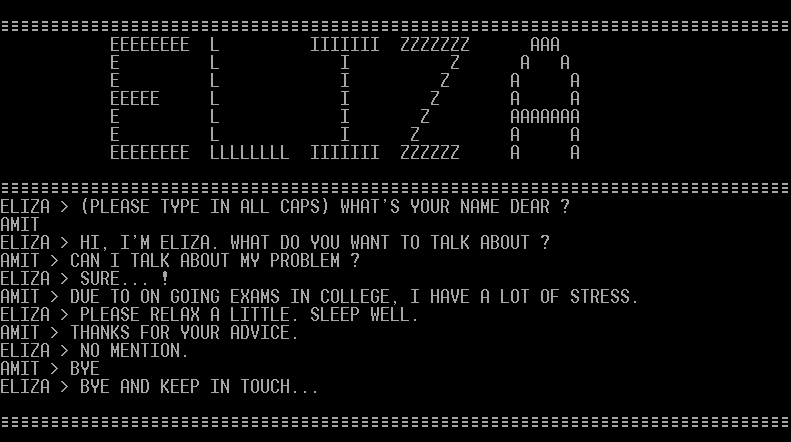
\includegraphics[width=\textwidth]{figures/eliza.png}
    \caption{Exemple de dialogue avec Eliza, le tout premier chatbot~\cite{Eliza}}
    \label{Eliza}
\end{figure}

Il existe aujourd'hui deux types d'agent conversationnel. Le premier repose sur un set de règles précises uniquement, et a donc un intérêt très limité puisqu'une seule formulation un peu exotique perdrait rapidement le bot. En revanche, le second type repose sur deux choses : des règles et l'intelligence artificielle. Tout d'abord, on inculque à notre robot une série de règles lui permettant d'identifier et de réagir à certains comportements précis de l'utilisateur. Ensuite, c'est la part d'intelligence artificielle qui pourra reconnaître d'autres comportements, en les comparant avec tout ce qu'elle connaît déjà, pour en déduire la réponse adaptée. Ce nouvel échange sera ajouté aux règles (\emph{machine learning}), qui seront donc de plus en plus fiables à chaque apprentissage de l'agent. Ce type de bot devient donc meilleur à chaque nouvelle interaction, et c'est pourquoi il est privilégié de manière générale. Vous pouvez trouver un schéma explicatif du processus de \emph{machine learning} ci-dessous [fig. \ref{Machine Learning}].\\

\begin{figure}[h!]
    \centering
    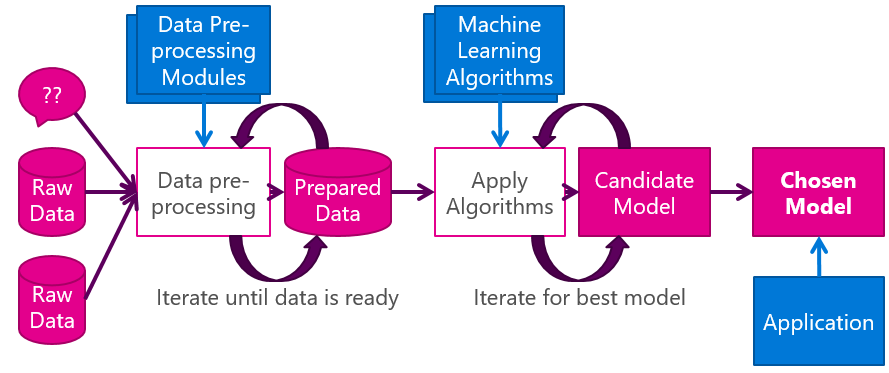
\includegraphics[width=\textwidth]{figures/machine learning.png}
    \caption{Schéma explicatif du processus de \emph{machine learning}~\cite{ML}}
    \label{Machine Learning}
\end{figure}



\section{Projet confié pendant le stage}

Lors de ce stage, ma tâche était donc de développer un agent conversationnel intégré dans l'application Mattermost [fig. \ref{MM}]. Mon bot devait pouvoir s'intégrer dans un canal avec plusieurs utilisateurs et se manifester lorsque son aide peut s'avérer utile, comme pour transmettre des informations précédemment données, rappeler une horaire de réunion,... \\

\begin{figure}[h!]
    \centering
    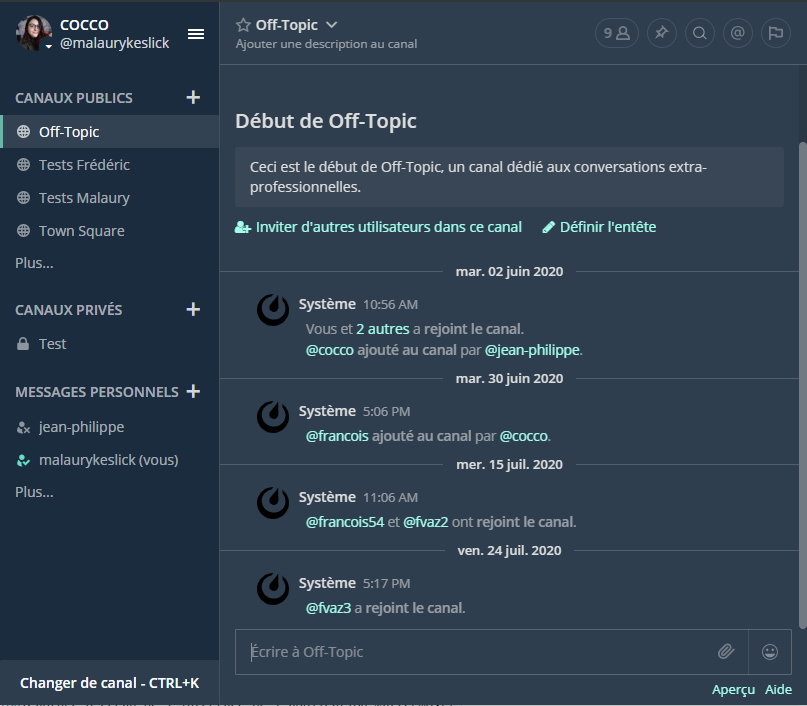
\includegraphics[width=\textwidth]{figures/Mattermost.PNG}
    \caption{Capture d'écran de l'interface de l'application Mattermost}
    \label{MM}
\end{figure}

Le développement était idéalement demandé en NodeJS ou en Python, et j'ai pour ma part choisi la première option. Finalement, comme expliqué précédemment, j'ai pour ma part utiliser les services cognitifs de Google Cloud pour mener à bien mon projet. 

\clearpage

\chapter{Réalisation et validation}

\section{Environnement matériel et logiciel}

Sur un total de neuf semaines de stage, j'en ai passé sept et demi en télétravail depuis mon domicile étudiant, à cause de la situation encore compliquée que présentait la crise de la COVID-19. J'ai choisi d'aller sur site pour la fin de mon stage afin de récupérer une ambiance de travail et un cadre sérieux, ce qui commençait à me manquer chez moi. J'ai effectué la totalité de mon travail depuis mon ordinateur personnel, un Dell Inspiron 5000 17 pouces, ce grand écran s'étant avéré très pratique dans des conditions où je ne pouvais pas faire de double-écran. \\

Pour travailler, j'ai essentiellement travaillé sur la plateforme de Google Cloud, utilisé l'éditeur de texte Atom et GitLab comme outil de gestion des versions. 

\section{Prise en main de Google Cloud et ses API}

\emph{Google Cloud Platform (GCP)} est une plateforme fournissant près d'une centaines de produits/services informatiques aux entreprises, professionnels de l'informatique et développeurs. Le cloud computing permet d'utiliser des produits et logiciels alors qu'ils existent dans des centres de données distants. Les utilisateurs peuvent donc y avoir accès depuis une interface en ligne comme la GCP, ce qui présente de nombreux avantages. Tout d'abord, aucun produit n'a besoin d'être installé directement sur la machine de l'utilisateur, et ainsi elle ne perd pas en stockage et en efficacité. D'autre part, la facilité de création d'un projet Google Cloud mêlant plusieurs services est indéniable, et la gestion des accès est également très simple d'utilisation.\\

Travailler avec la GCP permet d'accéder aux services de plus de cinquante API (\emph{Application Programming Interface}) allant de l'accès au stockage à l'analyse d'images basées sur le \emph{machine learning}. Dans le cadre de ce projet, j'ai eu recours aux API \emph{Cloud Functions} et \emph{Dialogflow}, et j'ai en parallèle utilisé le service \emph{Firebase} permettant d'intégrer une base de données en temps réel à mon application. 

\subsection{Google Cloud Functions}
\emph{Google Cloud Functions} (GCF) est une solution FaaS (\emph{Functions as a Service}) permettant de créer des fonctions répondant aux événements cloud sans avoir à gérer ni de serveurs ni d'environnements d'exécution~\cite{GCF}. C'est le service que j'ai utilisé pour gérer deux axes de mon projets : \\
\begin{itemize}
    \item l'intégration de mon chatbot dans Mattermost ;
    \item la gestion des réponses (\emph{fulfillment}) de mon bot à un type de message en particulier (cette partie sera plus amplement explicitée dans la prochaine partie).
\end{itemize}
\subsection{Dialogflow}
\emph{Dialogflow} est l'outil majeur que j'ai utilisé lors de ce stage. C'est une plateforme permettant la création et l'intégration d'agents conversationnels au sein d'applications mobiles et Web, de système de réponse vocale interactive,... Ce système peut analyser les entrées provenant de clients (qu'elles soient audio ou textuelles) et répondre de différentes manières en fonction de la manière dont il est programmé. \\

Lorsque \emph{Dialogflow} reçoit une entrée, il la compare aux ``intents'' qu'ils lui ont été enseignés. Un intent comprend un titre, éventuellement des contextes [fig. \ref{contexts}], des phrases d'entraînement [fig. \ref{trainingphrases}], d'éventuels paramètres [fig. \ref{responses1}] et enfin des réponses [fig. \ref{responses1}]. Nous allons ici voir l'utilité de chacun de ces éléments via l'intent ``Présentation''. Il existe deux types de contextes : les sortants qui permettent d'indiquer au système qu'il doit retenir l'une des informations qu'on lui a fourni, et ce pendant un certain nombre de tours ; et les entrants qui indique quel est l'élément (qu'il est censé déjà connaître) qu'il doit récupérer pour le réutiliser dans la suite du processus. \\
\begin{figure}[h!]
    \centering
    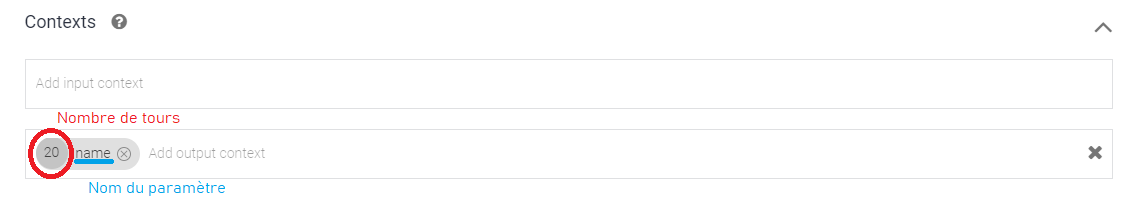
\includegraphics[width=\textwidth]{figures/contexts.PNG}
    \caption{Exemple de contexte pour l'intent ``Présentation''}
    \label{contexts}
\end{figure}

Ensuite, on donne à l'intent quelques phrases types reflétant ce que l'utilisateur pourrait dire, et l'on repère les mots-clés importants par un type d'entité. Différentes entités sont déjà existantes dans \emph{Dialogflow}, comme les dates, les villes,.. et l'on peut en créer de nouveaux personnalisés, comme par exemple des salles de réunions, des types d'événements.. comme l'indique l'exemple suivant [fig. \ref{entity}].\\
\vspace{2\linewidth}
\begin{figure}[h!]
    \centering
    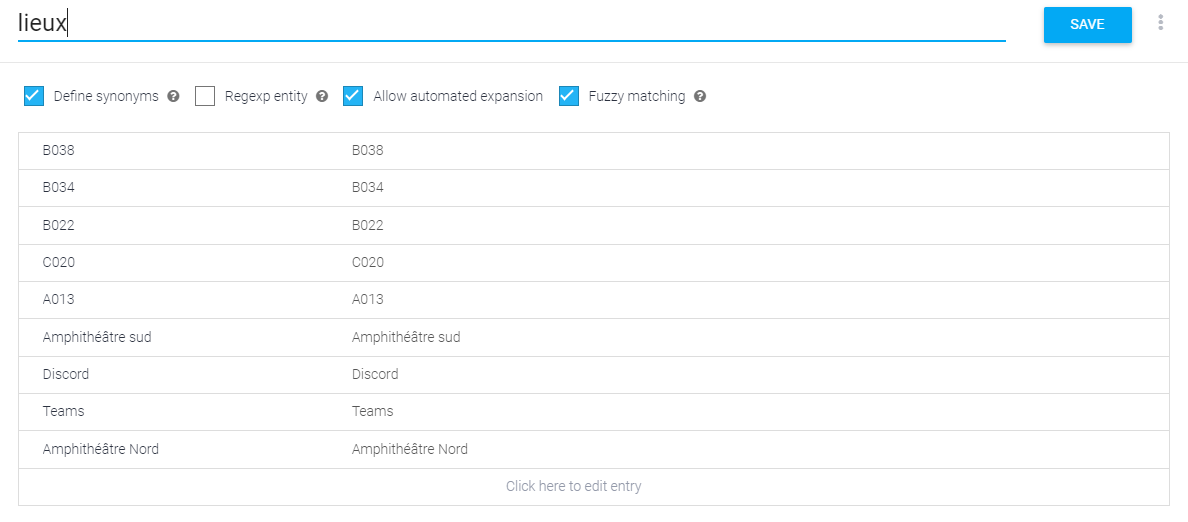
\includegraphics[width=\textwidth]{figures/entity.PNG}
    \caption{Exemple d'entité pour les différents lieux (réels ou virtuels) d'événements}
    \label{entity}
\end{figure}

Voici ainsi un exemple de phrases d'entraînements que j'ai fournies dans le cadre de mon intent "Présentation".\\
\begin{figure}[h!]
    \centering
    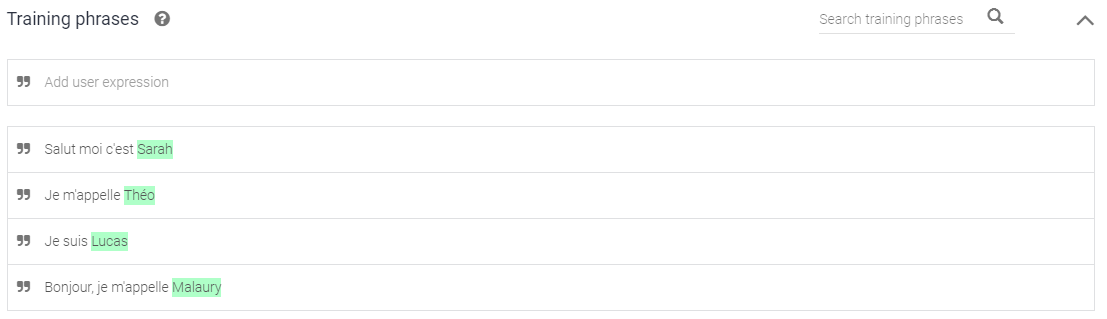
\includegraphics[width=\textwidth]{figures/trainingphrases1.PNG}
    \caption{Exemples de phrases d'entraînement pour l'intent ``Présentation''}
    \label{trainingphrases}
\end{figure}



\`{A} partir de ces éléments, lorsqu'un utilisateur saisit l'une de ces phrases (ou quelque chose y ressemblant), le système reconnaît le nom de l'utilisateur et pourra alors produire des réponses personnalisés. Grâce aux contextes précédemment présentés, il pourra d'ailleurs le retenir pendant 20 tours après la saisie de cette phrase. \`{A} noter qu'il existe la case ``Required'' dans la liste des paramètres, comme vous pouvez le voir ci-dessous, qui sert à exiger une information. Ainsi, si elle n'est pas donnée, on peut programmer un message qui pourrait être ici ``Bonjour! Comment t'appelles-tu?''. Pour répondre à l'utilisateur, il existe alors plusieurs options. La première, que nous allons voir ici, est utilisable lorsque la réponse ne dépend pas des expressions entrées par l'utilisateur. Par exemple dans notre cas, le système aura un panel de réponses toutes faites à renvoyer, et ce peu importe le prénom entré.  \\
\begin{figure}[h!]
    \centering
    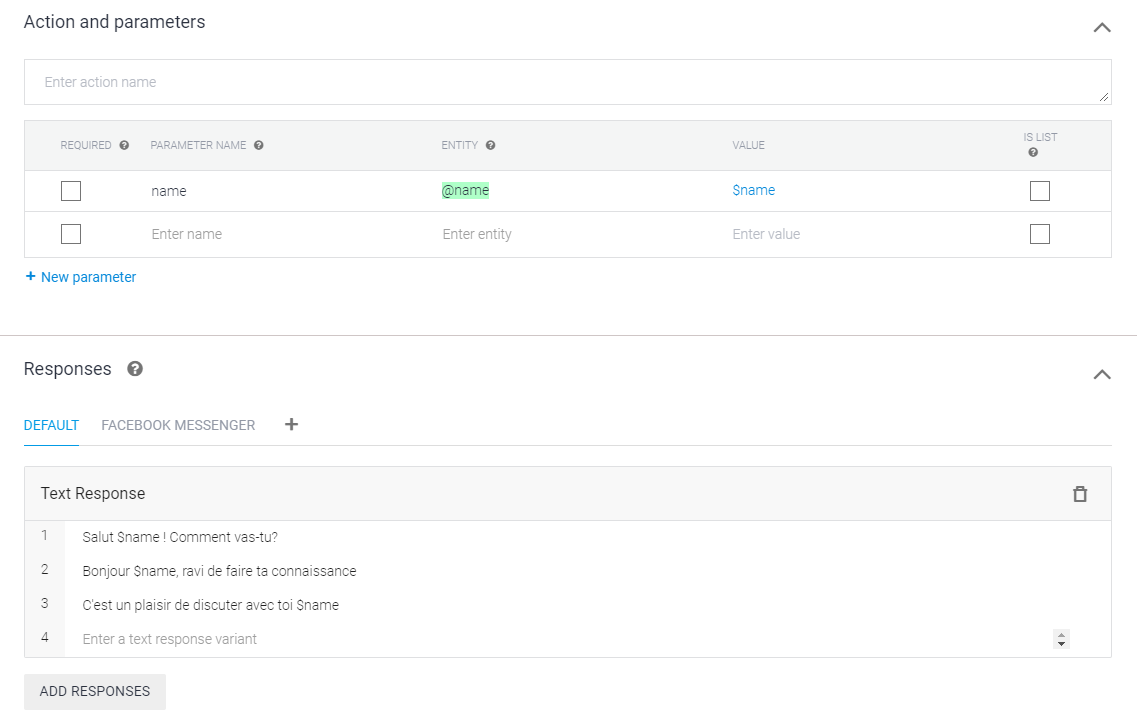
\includegraphics[width=\textwidth]{figures/responses1.PNG}
    \caption{Démonstration de l'utilisation des expressions dans le cadre de réponses simples pour l'intent ``Présentation''}
    \label{responses1}
\end{figure}

\vspace{\linewidth}
Dans le cas où l'on doit travailler sur les différents paramètres avant de pouvoir produire une réponse (ou si l'on doit faire une entrée dans la base de données \emph{Firebase} par exemple), il faut alors autoriser les appels au webhook disponible dans la partie fulfillment de \emph{Dialogflow}. Le webhook en question est une \emph{Google Cloud Function}, qui reçoit une requête HTTP provenant du client avec les éléments entrés par l'utilisateur sous format JSON. C'est ce qui va permettre par exemple, de déterminer si la date entrée est valide, si la salle de réunion demandée est disponible à l'instant t, d'entrer des informations dans la base de données.. \\

Je vais maintenant vous présenter les différents intents que j'ai créés dans le cadre de ce stage, et les éventuelles fonctions de fulfillment associées.

\subsubsection{Programmation d'un événement}

Pour ce projet, je me suis concentrée sur des échanges d'informations à propos d'évènements au sein d'une équipe ou d'une entreprise. Ainsi, j'ai créé une entité \emph{event} [fig. \ref{event}], afin que mon système puisse reconnaître les différentes catégories pouvant exister. Un utilisateur de mon bot peut donc choisir de programmer une réunion, une conférence ou une visio-conférence.\\

\begin{figure}[h!]
    \centering
    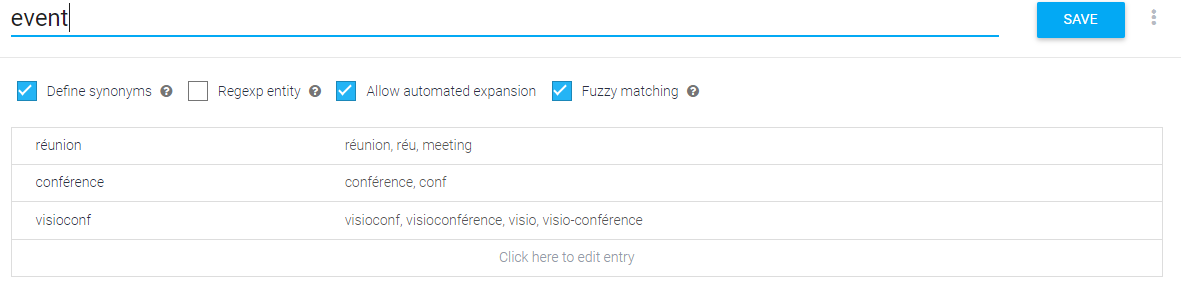
\includegraphics[width=\textwidth]{figures/entities2.PNG}
    \caption{Entité \emph{event} créée pour la programmation d'évènement}
    \label{event}
\end{figure}

\vspace{\linewidth}
Afin de pouvoir programmer ces différentes catégories d'évènements, j'ai eu besoin de créer deux autres entités, les lieux et le nom du bot. La première sert à ce que mon robot reconnaisse un nom de salle, d'amphithéâtre, ou même la plateforme utilisée si l'évènement se produit à distance. J'ai choisi d'utiliser des exemples réalistes dans le cadre de mon équipe au Loria (notamment au niveau des noms de salle) et de la situation actuelle (réunion en visio), mais c'est quelque chose qui peut être très facilement ajustable en ajoutant de nouveaux exemples dans cet entité. Cet entité a déjà été présentée un peu plus haut [fig. \ref{entity}].\\

Ensuite, l'entité responsable du nom du bot est celle qui permettra au bot de comprendre si l'on parle de lui a un moment donné dans une phrase, ou si l'on cherche à le mentionner pour s'adresser directement à lui [fig. \ref{BotName}]. Dans le cadre de ce stage, j'ai choisi de lui donner un nom générique (\emph{chatbot}) mais il est bien sûr personnalisable en allant le modifier directement dans l'entité et dans les paramètres d'intégration.\\

\begin{figure}[h!]
    \centering
    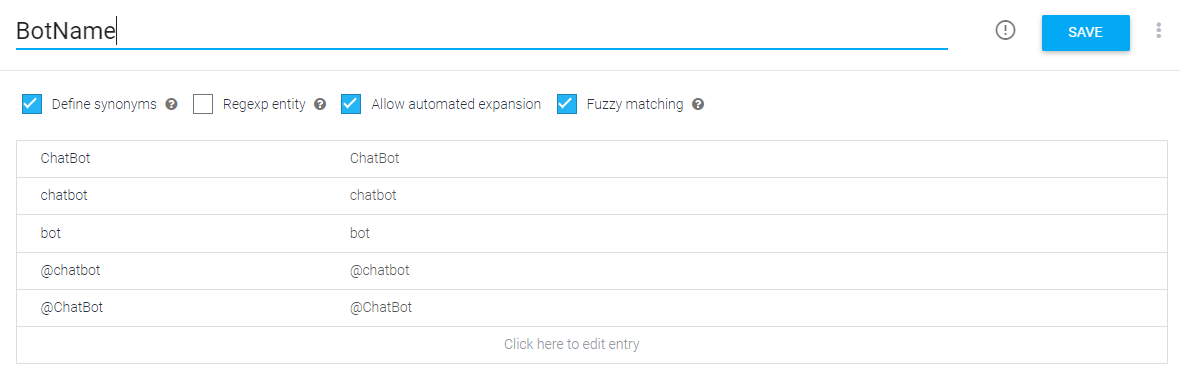
\includegraphics[width=\textwidth]{figures/botname.PNG}
    \caption{Entité \emph{BotName} créée pour le dialogue avec le bot}
    \label{BotName}
\end{figure}
\vspace{\linewidth}

Ces entités créées de toute pièce, plus l'entité déjà connue par \emph{Dialogflow}, \emph{@sys.date-time} responsable de la reconnaissance de dates et heures, m'ont permis de créer l'intent \emph{EventHandling}. Cet intent est celui qui me permet de reconnaître la volonté d'un utilisateur de programmer un évènement. Si au départ je n'avais pris en compte que le cas où l'on s'adressait directement au Bot, j'ai ensuite rajouté le cas où ces informations se glissent au sein d'une conversation entre plusieurs utilisateurs. Voici un aperçu des phrases d'entraînement que j'ai soumises à mon système [fig. \ref{EHtp}]:\\

\begin{figure}[h!]
    \centering
    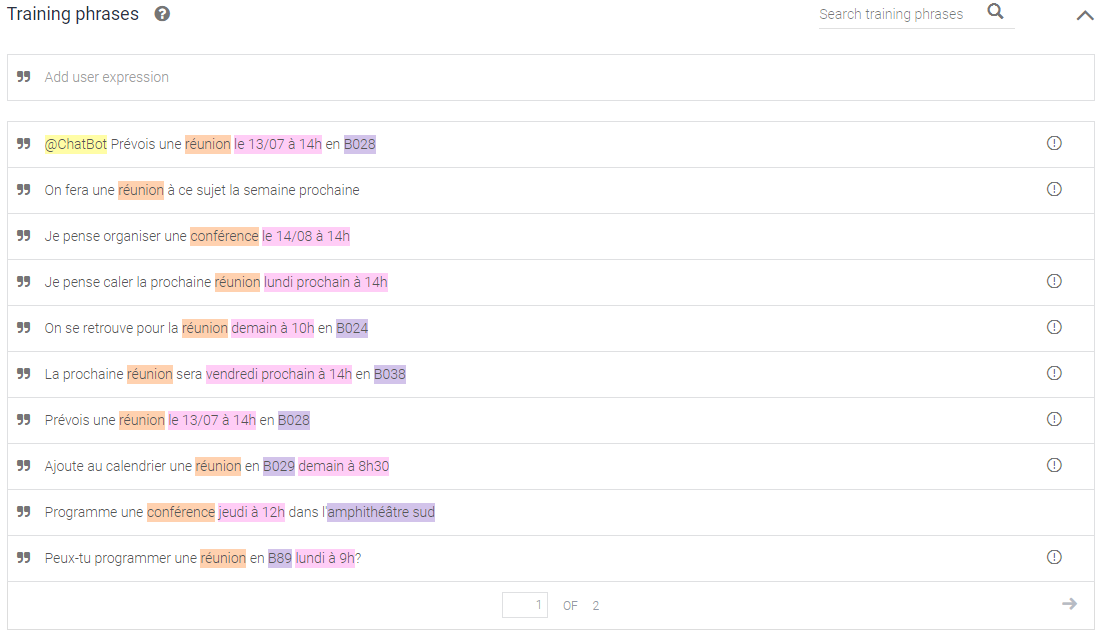
\includegraphics[width=\textwidth]{figures/EHtraining.PNG}
    \caption{Phrases d'entraînement pour l'intent \emph{EventHandling}}
    \label{EHtp}
\end{figure}


Il s'agit ensuite pour le bot de s'assurer qu'il a bien recueilli toutes les informations nécessaires pour discriminer un évènement, c'est-à-dire son type, son lieu, et sa date (jour et heure, sachant que si l'horaire n'est pas précisée, elle sera automatiquement à 12h). Si le système se rend compte qu'il lui manque l'une de ces informations, une \emph{prompt phrase} est alors envoyée à l'utilisateur, lui demandant le paramètre manquant [fig \ref{prompt}]. \\

\begin{figure}[h!]
    \centering
    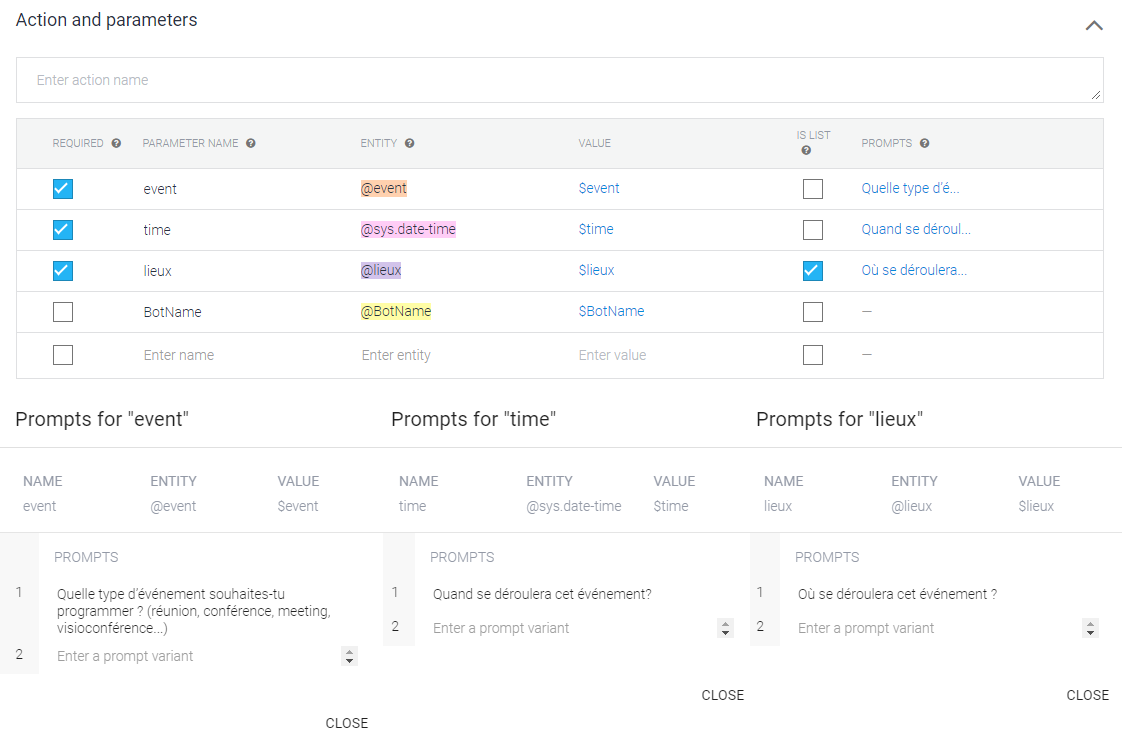
\includegraphics[width=\textwidth]{figures/EHparameters.png}
    \caption{Paramètres et \emph{prompt phrases} pour l'intent \emph{EventHandling}}
    \label{prompt}
\end{figure}

Une fois tous les paramètres reçus, ces informations sont envoyées sous format JSON à la partie \emph{fulfillment} de l'application. Ma \emph{Google Cloud Function} responsable de cette partie est écrite en NodeJS, et repose essentiellement sur le package \emph{dialogflow-fulfillment}, qui permettra d'envoyer une réponse au système. J'utilise également le service Google \emph{Firebase} afin d'avoir une base de données en temps réel des évènements ajoutés au calendrier. Cette partie sera détaillée un peu plus tard [section 4.2.3].\\

Ainsi, une fois les informations reçues dans la requête, une nouvelle entrée est créée dans la base de données. J'aurais aimé que le système vérifie si la date est valide, que l'évènement en question n'ait pas déjà été programmé et enfin que la salle demandée soit disponible à ce moment-là avant d'écrire dans la base, mais j'ai rencontré quelques problèmes en Javascript qui m'en ont empêché. Je présenterai ce problème dans mon bilan [section 5]. \\

\subsubsection{Demande d'informations à propos d'un événement}

Une fois des évènements ajoutés à la base de données, nous voulons naturellement pouvoir en lire les informations. Ainsi, un utilisateur peut se poser diverses questions, par exemple sur l'heure d'une réunion, sur la disponibilité d'une salle, sur le programme d'une journée en particulier... C'est ce que contrôle mon intent \emph{ReadFromDB}, dont les phrases d'entraînement vous sont présentées ci-dessous [fig. \ref{RFDBtrain}].\\

\begin{figure}[h!]
    \centering
    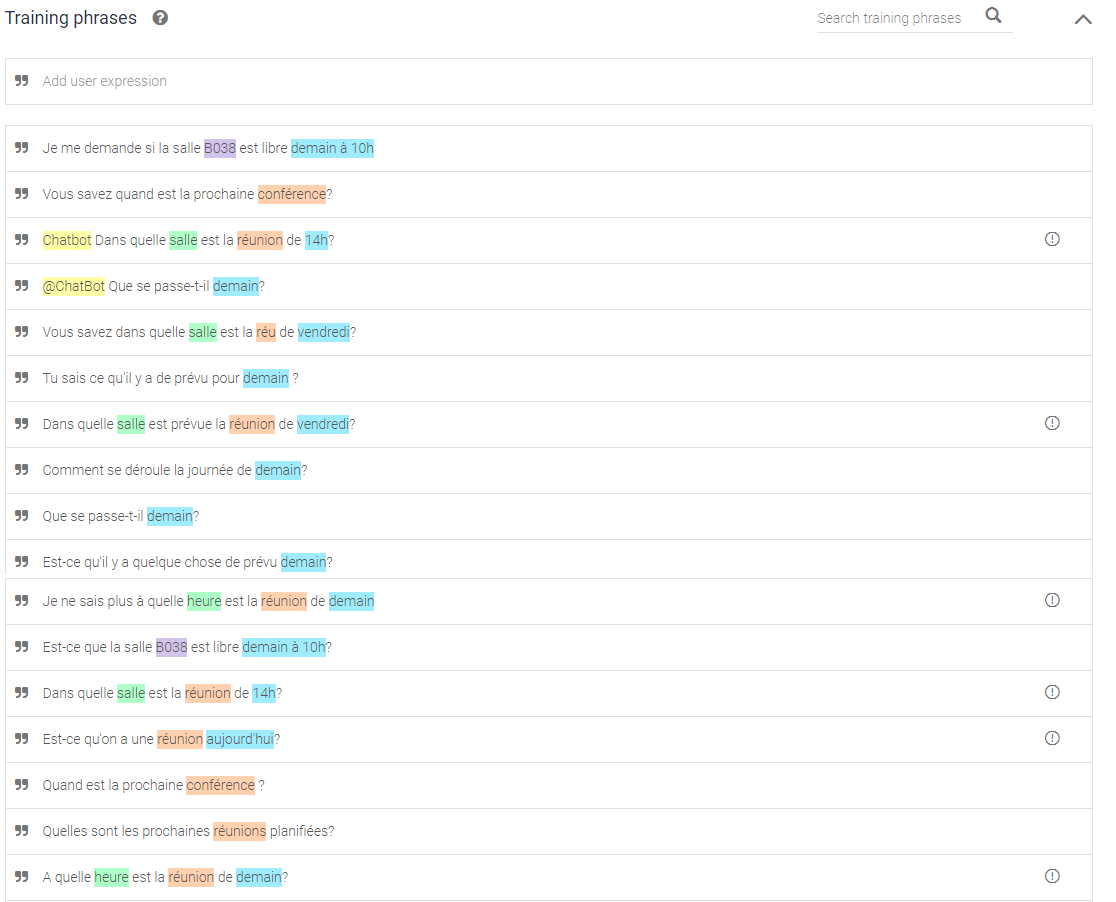
\includegraphics[width=\textwidth]{figures/RFDBtraining.png}
    \caption{Phrases d'entraînement pour l'intent \emph{ReadFromDB}}
    \label{RFDBtrain}
\end{figure}

Dans ce cas de figure, aucun paramètre n'est requis, puisque l'analyse de l'information voulue se fera sur le nombre et le type de paramètres proposés par l'utilisateur. J'ai ici rajouté un paramètres de l'entité système \emph{@sys.any} qui me permet de reconnaître quand certaines informations très précises sont demandées, par exemple une heure ou un lieu. Comme le montre la correspondance du tableau suivant [fig. \ref{RFDBparam}], ces paramètres sont surlignés en vert dans les phrases d'entraînement précédentes. Ce nouveau paramètre me servira dans la distinction faite dans la partie fulfillment, lorsque le bot cherchera à comprendre quelle est l'information recherchée.\\

\begin{figure}[h!]
    \centering
    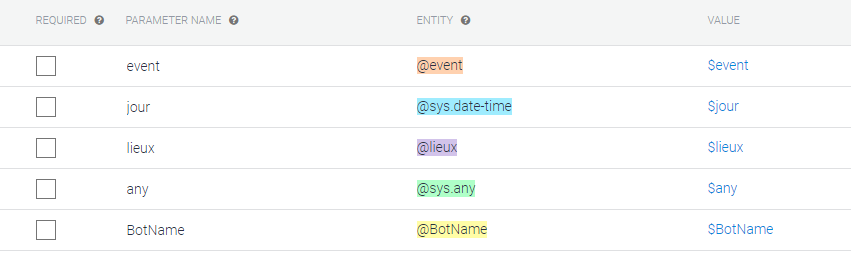
\includegraphics[width=\textwidth]{figures/RFDBparam.PNG}
    \caption{Paramètres pour l'intent \emph{ReadFromDB}}
    \label{RFDBparam}
\end{figure}

\clearpage

En fonction des paramètres reçu, on peut chercher à déterminer ce que l'utilisateur souhaite savoir : \\
\begin{itemize}
    \item si seul le type d'évènement est renseigné, alors le système répondra à la question "Quand est le prochain [type d'évènement]?" ;
    \item si seule la date est renseignée, alors le système répondra à la question "Quel est le programme du [jour donné]?" ;
    \item si la date (sous-entendu avec l'heure) et le lieu sont donnés, alors le système répondra à la question "Est-ce que [lieu] est disponible le [date]?" ;
    \item et enfin si un paramètre \emph{@sys.any} a été reconnu, c'est alors que les champs type et date ont également été remplis, et le système répondra à une question du type "A quelle heure/dans quelle salle est la réunion de demain?".\\
\end{itemize}

Cette fonction requiert de lire dans la base de données \emph{Firebase}, ce mécanisme sera explicité un peu plus tard.

\subsubsection{Modification d'une entrée dans la base de données}

Il peut également arriver qu'un utilisateur souhaite modifier l'heure, la salle de de rendez-vous pour un évènement en particulier. C'est l'intent \emph{ModifyDB} qui se charge de repérer cet intention chez l'utilisateur. De nouveau, le pannel des phrases d'entraînement est assez large pour aller de l'adressage direct au bot à du repérage même au sein d'une conversation entre collègues [fig. \ref{modify}].\\

\begin{figure}[h!]
    \centering
    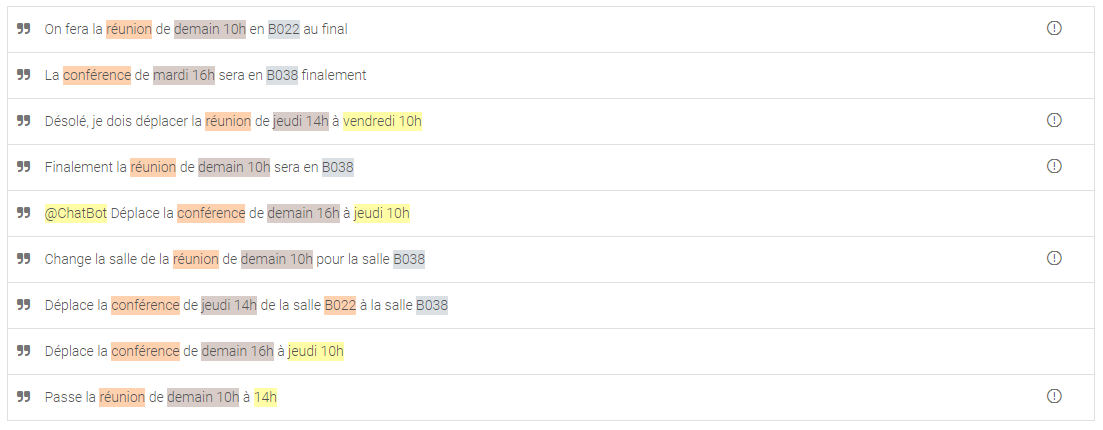
\includegraphics[width=\textwidth]{figures/MDBtrain.PNG}
    \caption{Phrases d'entraînement pour l'intent \emph{ModifyDB}}
    \label{modify}
\end{figure}

Le procédé est alors le suivant : on récupère les informations nécessaires à la discrimination de l'évènement à modifier, puis l'on parcourt la base de données à la recherche de l'entrée correspondante. On récupère alors toutes les informations, on actualise celles demandées, on supprime l'entrée initiale avant de soumettre une nouvelle entrée ayant l'identifiant de la précédente, avec la mise à jour. Si jamais on ne rencontre jamais l'évènement demandé dans la base, on prévient alors l'utilisateur qu'aucune correspondance n'a été trouvée.



\begin{figure}[h!]
    \centering
    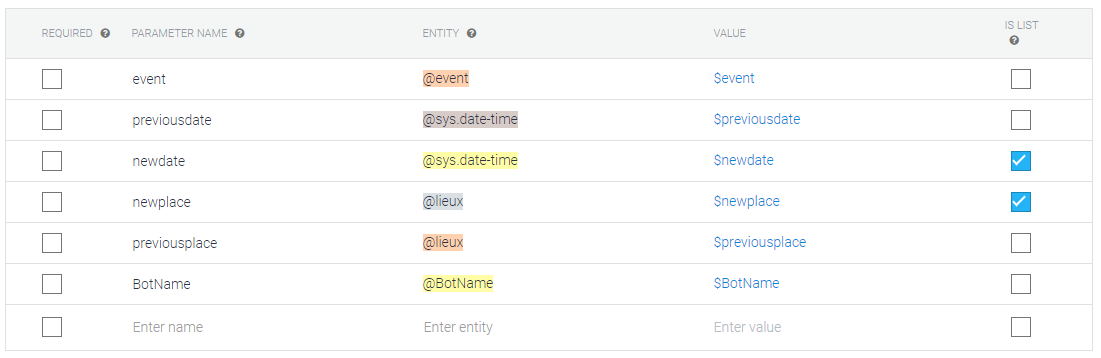
\includegraphics[width=\textwidth]{figures/MDBparam.PNG}
    \caption{Paramètres pour l'intent \emph{ModifyDB}}
    \label{modifyParam}
\end{figure}

\vspace{\linewidth}

\subsubsection{Les fonctions annexes}

Pour mener à bien mon travail et rendre le résultat final plus confortable à l'utilisateur, j'ai eu besoin de développer quelques petites choses en plus :\\
\begin{itemize}
    \item la conversion des format horaires système (2020-06-18T14:00:00+02:00) en quelque chose de facilement compréhensible pour l'utilisateur (jeudi 18 juin à 14h) ;
    \item la réponse à la question "Qu'est-ce que tu peux faire pour moi?" et ses reformulations, afin que les utilisateurs puissent être guidés sur ce que le bot peut leur apporter.\\
\end{itemize}

\vspace{13\baselineskip}

\subsection{Firebase Realtime Database}

\emph{Firebase} propose un service de base de données NoSQL stockée dans le cloud Google : \emph{Firebase Realtime Database}. Il permet de relier une application (en l'occurrence le chatbot) a une base de données en temps réel, accessible par tous les utilisateurs (ou pas si l'on souhaite configurer les règles d'accès en lecture et/ou écriture de manière spécifique). Initialement, une variable globale nommée ID est initialisée à 0 dans le code gérant la partie \emph{fulfillment}. Avant chaque écriture dans la base, on incrémente cette variable afin que chaque évènement enregistré ait un identifiant unique. Ces identifiants serviront notamment lors de la lecture de la base (pour créer une boucle sur le nombre d'éléments présents), mais aussi pour la modification des informations, puisque l'on saura ainsi précisément quelle entrée supprimer, ainsi que sa position pour le réinsérer dans la base de données. L'interface de \emph{Firebase} me permettait de pouvoir suivre l'évolution en temps réel, et je pouvais enfin m'assurer du bon déroulement des opérations [fig. \ref{firebase}].\\

\begin{figure}[h!]
    \centering
    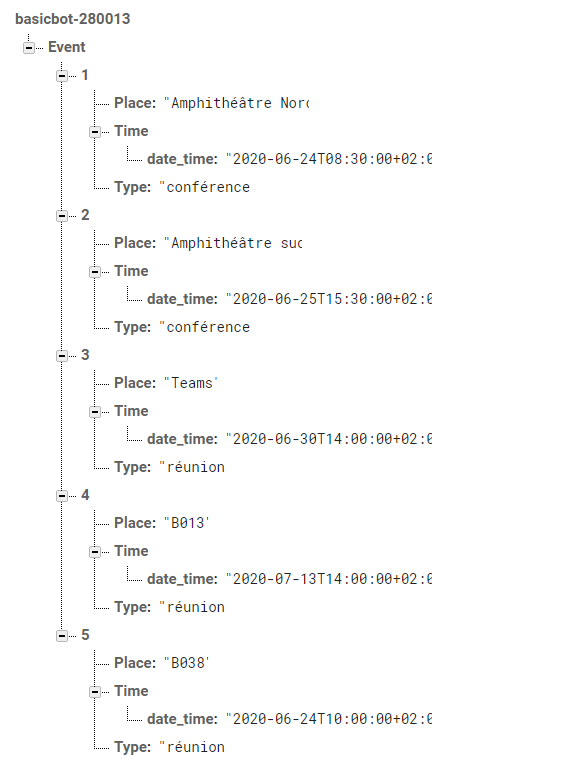
\includegraphics[width=0.9\textwidth]{figures/Firebase.png}
    \caption{Interface de la base de données à temps réel \emph{Firebase}}
    \label{firebase}
\end{figure}

\newpage

\section{Intégration du bot dans Mattermost}

Même si je ne suis pas parvenue à intégrer mon bot dans Mattermost, je vais ici vous présenter la théorie de son fonctionnement. Pour cela, je vais me reposer sur le schéma proposé dans la documentation de l'API \emph{Dialogflow}~\cite{APIdialogflow}[fig. \ref{API}].\\

\begin{figure}[h!]
    \centering
    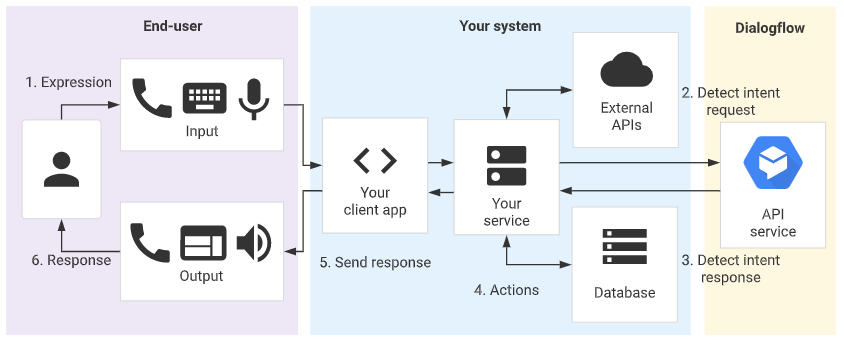
\includegraphics[width=\textwidth]{figures/API_schema.PNG}
    \caption{Fonctionnement global de l'intégration d'un chatbot~\cite{APIdialogflow}}
    \label{API}
\end{figure}

La partie intégration réside dans la case centrale ``\emph{Your client app}''. En effet, si \emph{Dialogflow} propose une intégration quasiment directe avec nombre d'applications existantes (Slack, Twitter, Messenger, Kik,...), lorsque ce n'est pas le cas comme avec Mattermost, il faut passer par du code. L'idée est que notre application client serait une \emph{Google Cloud Function}, deployée dans le même projet que le projet \emph{Dialogflow} précedemment présenté. On relierai alors cette fonction à Mattermost en récupérant son \emph{trigger URL} via l'interface de GCP, puis on irait la copier dans la section URLs de callback du webhook sortant crée dans la partie intégration de l'application Mattermost [fig. \ref{wh}]. \\

\begin{figure}[h!]
    \centering
    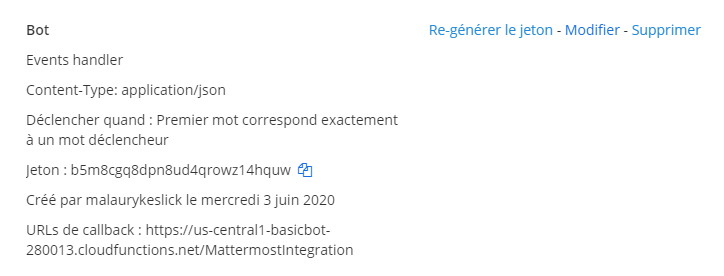
\includegraphics[width=\textwidth]{figures/MattermostWebhook.PNG}
    \caption{Affichage de la section \emph{Outgoing Webhooks} de Mattermost}
    \label{wh}
\end{figure}

\vspace{\linewidth}
Le jeton présenté [fig. \ref{wh}] peut être utilisé pour augmenter la sécurité de l'application et s'assurer que les requêtes envoyé à URL de la GCF proviennent exclusivement de ce webhook. Les informations alors transmises via Mattermost seront envoyées au format JSON à cette URL de callback, et la GCF correspondante se chargera de les transmettre à \emph{Dialogflow}, qui travaillera sur les données avant de renvoyer une réponse au client, qui le renverra lui-même à Mattermost.\\

Puisque je n'ai personnellement pas réussi à mener à bien cette opération, j'ai intégré mon robot à l'application Slack, puisque les possibilités offertes par \emph{Dialogflow} et l'API Slack rendaient l'intégration assez simple. Ce choix me semblait pertinent à deux niveaux. Tout d'abord, Mattermost est une alternative open-source de Slack, et donc j'espère qu'avoir réussi à rendre mon travail fonctionnel sur l'un permettra la même chose sur le second. De plus, Slack permet, tout comme Mattermost, de créer des canaux de conversation de groupe, et ainsi j'ai pu tester et développer tout ce que je voulais faire sur cette application sans soucis. \\ 

\section{Scénarios d'échange avec le bot}
Dans cette partie, je vais vous présenter quelques scénarios d'échange avec mon bot, regroupant la totalité de ce qu'il est possible de faire grâce à celui-ci. Dans le premier cas, je donne l'exemple du lancement du bot [fig. \ref{sc1}], lorsque la base de données étant encore vide [fig. \ref{db1}]. Dans le deuxième scénario, j'ai préalablement ajouté un nombre conséquents d'évènements à la base de données [fig. \ref{db2}] afin de pouvoir poser des questions plus intéressantes et illustrer l'étendue de ce dont mon chatbot est capable [fig. \ref{sc2}].\\
\begin{figure}[H]
    \centering
    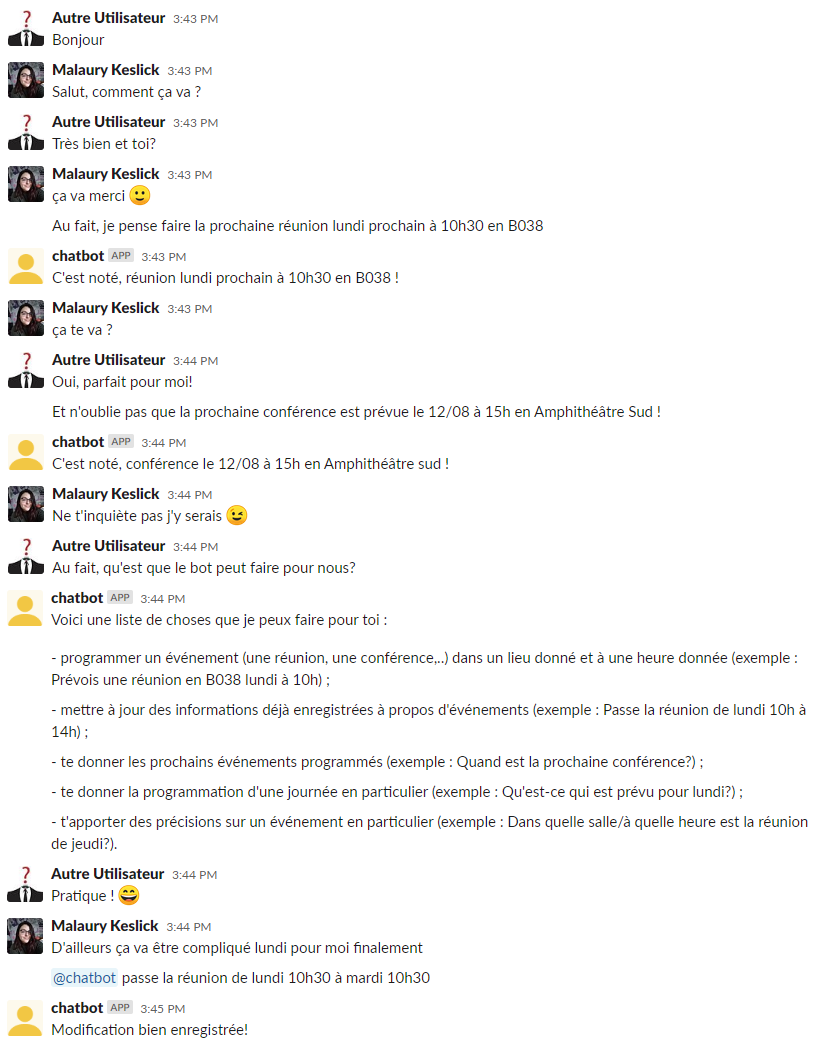
\includegraphics[width=\textwidth]{figures/scenario1.png}
    \caption{Scénario d'échange chatbot - utilisateurs numéro 1}
    \label{sc1}
\end{figure}

\begin{figure}[H]
    \centering
    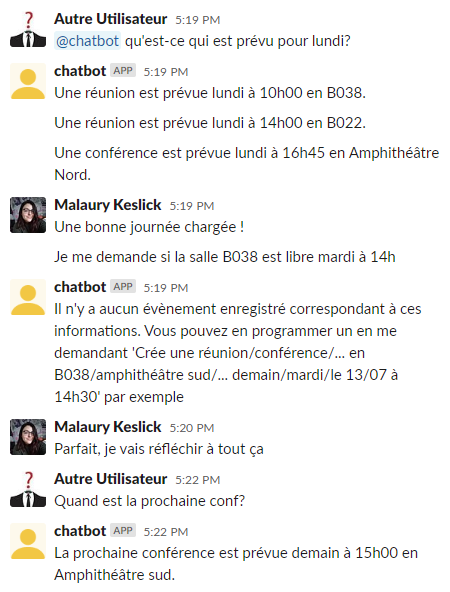
\includegraphics{figures/scenario2.PNG}
    \caption{Scénario d'échange chatbot - utilisateurs numéro 2}
    \label{sc2}
\end{figure}

\section{Limites et développements futurs}

\subsection{Optimisation du bot}
TODO une fois la partie du dessus bouclée\\
réussir à mettre au point les conditions d'écriture dans la DB \\
Gérer le multi-users (pour que le bot sache de qui il attend une réponse et ne panique pas si quelqu'un d'autre parle entre temps, gestion du cas si c'est un autre utilisateur qui répond a sa question)\\
notion de hiérarchie entre les users\\
regarder dans le doc d'avancée si y'a d'autres trucs intéressants\\
système de notifs \\
ajout de fonctionnalités comme la traduction via réaction -> pratique pour les équipes multilingues (lien?)\\

\subsection{Lien avec d'autres outils Google}
On pourrait songer à voir le bot connecté avec plusieurs outils Google afin de rendre son utilisation entre plus agréable et efficace. Par exemple, à la place d'utilise \emph{Firebase}, on pourrait choisir de relier directement le chatbot au \emph{Google Agenda} de l'équipe concerné. Ainsi les participants verraient leur emploi du temps automatiquement mis à jour et recevraient des notifications à l'approche des évènements. On pourrait également songer à le relier à \emph{Google Meet} afin d'y planifier les visio-conférences automatiquement. Dans un autre registre que celui de la programmation d'évènements, on pourrait le relier à \emph{Google Drive}, pour de la recherche de fichiers efficace ; à \emph{Gmail}, pour retrouver rapidement la date d'un mail, le transférer, retrouver un ordre du jour... \\
Les fonctions Google sont presque illimitées, et ainsi il serait possible de réaliser un chatbot très complet grâce à ces outils.

\subsection{Sécurité}
Je n'ai pas eut le temps de me pencher dessus, mais la question de la sécurité serait intéressante à traiter pour ce type d'application. D'une part, il faudrait être sûr que personne ne puisse venir lire ou altérer les données dans la base \emph{Firebase} directement, puisqu'elle pourrait contenir des informations cruciale pour des personnes hostiles à l'entreprise. D'autre part, même si l'accès à la base de données est sécurisé, il faudrait aussi s'assurer que le système ne peut pas recevoir de requêtes HTTP de n'importe qui, puisque le bot pourrait alors communiquer des informations confidentielles, ou même être complètement détourné de son utilisation initiale.

\clearpage

\chapter{Bilan}

%Plan : \\
%Avis de Mr Charoy et Clélie \\
%Continuité du projet (PI officialisé?)\\
\`{A} propos des difficultés rencontrées pendant ce stage, je dirais que la principale était la condition de télé-travail pendant la quasi-totalité de mon expérience, et surtout au début. Il m'a été difficile de juger de mon avancée par moi-même, et il était parfois difficile de différencier les moments de travail des moments de détente au sein de mon logement étudiant. C'est pourquoi j'ai choisi de finalement revenir sur site pour la fin de mon stage, afin d'être plus cadrée, avec des horaires fixes et une bonne atmosphère de travail. \\

D'un côté plus technique, j'ai du faire face à la découverte d'un nouveau langage de programmation, le Javascript. Si dans un premier temps cela ne m'a pas trop posé de problèmes, puisque nous sommes bien formés à nous adapter facilement à l'école, j'ai fini par me heurter à une difficulté majeure. En effet, c'était la première fois que je rencontrais de la programmation asynchrone, si bien que j'ai d'abord mis un long moment à comprendre d'où venait mon problème lorsque j'essayais de travailler sur les conditions d'écriture dans la base de données. Après quelques recherches sur le sujet et quelques tentatives de résolution de mon problème, j'ai du abandonner cette option par manque de temps restant. J'ai tout de même laisser mes pistes de réflexion et tentatives en commentaire dans mon code, afin que les personnes qui poursuivront ce projet puissent s'y référer. \\

De même, comme vous avez pu le remarquer dans ce rapport, j'ai fais face à une difficulté que je n'ai pas réussi à surmonter : celle de l'intégration de mon bot dans l'application Mattermost. J'ai longtemps tourné en rond car je me reposais sur des tutoriels qui ne fonctionnait qu'avec une ancienne version de Dialogflow. J'ai finalement trouvé de quoi travailler avec la version actuelle du service \cite{MMintegration}, mais je n'ai jamais réussi à mettre cela en place à cause de problème de package que j'avais pourtant installé dans mon projet. Ce point reste encore un mystère pour moi aujourd'hui, mais j'ai préféré intégrer mon chatbot dans Slack afin de ne pas me retarder encore plus, tout en pouvant tester les fonctionnalités de mon agent dans le contexte de conversations à plusieurs utilisateurs.\\

Les deux difficultés suivantes se sont révélées être d'excellentes surprises puisqu'elles m'auront beaucoup apporté lors de ces quelques semaines. Dans un premier temps je parlerai des technologies cloud, que je ne connaissais que de nom jusque-là. Si j'ai du beaucoup me renseigner pour comprendre l'ampleur de leur puissance, j'ai trouvé cela tellement fascinant que j'espère avoir l'occasion de travailler de nouveau avec ces outils dans ma carrière. \\

Enfin, ce stage aura été pour moi synonyme d'autonomie et de prise d'initiatives. Même si cela m'effrayait un peu au départ, j'ai trouvé cette manière de travailler très agréable et très formatrice. Cela m'aura appris à ne pas baisser les bras trop rapidement, et si la frustration de ne pas avancer est plus grande lorsque l'on est seule face à son écran, la satisfaction de réussir l'est encore plus. \\

Pour conclure ce bilan, je peux dire que même si le projet reste à retravailler, la base et les pistes d'amélioration présentées dans ce projet permettront à terme d'étudier la confiance dans la collaboration entre chatbots et humains. Le dépôt git utilisé lors de ce projet est organisé de manière à rendre la reprise du projet la plus agréable et efficace possible.\\

\clearpage

\comment{\chapter{Exemples Listings}

Il est aisé d'insérer du code dans un rapport. Il suffit de définir le langage, la légende à afficher et enfin un Label pour pouvoir y faire référence. Le résultat est donnée dans le listing \ref{lst:premierExemple}. Il est également possible de changer les couleurs, pour cela il faut éditer le lstset dans la classe tnreport.cls.

\begin{lstlisting}[language=c++, caption={Premier Exemple}, label={lst:premierExemple}]
void CEquation::IniParser()
{
	if (!pP){ //if not already initialized...
		pP = new mu::Parser;

		pP->DefineOprt("%", CEquation::Mod, 6); //deprecated
		pP->DefineFun("mod", &CEquation::Mod, false);
		pP->DefineOprt("&", AND, 1); //DEPRECATED
		pP->DefineOprt("and", AND, 1);
		pP->DefineOprt("|", OR, 1); //DEPRECATED
		pP->DefineOprt("or", OR, 1);
		pP->DefineOprt("xor", XOR, 1);
		pP->DefineInfixOprt("!", NOT);
		pP->DefineFun("floor", &CEquation::Floor, false);
		pP->DefineFun("ceil", &CEquation::Ceil, false);
		pP->DefineFun("abs", &CEquation::Abs, false);
		pP->DefineFun("rand", &CEquation::Rand, false);
		pP->DefineFun("tex", &CEquation::Tex, false);

		pP->DefineVar("x", &XVar);
		pP->DefineVar("y", &YVar);
		pP->DefineVar("z", &ZVar);
	}
}
\end{lstlisting}
\clearpage
Il est également possible d'afficher du code directement depuis un fichier source, le résultat de cette opération est visible dans le listing \ref{lst:fromSrc}
\lstinputlisting[language=c++,caption={Affichage depuis le fichier source},label={lst:fromSrc}]{figures/sourceCode.cpp}

De nombreux languages sont supportés : \\
ABAP2,4, ACSL, Ada4, Algol4, Ant, Assembler2,4, Awk4, bash, Basic2,4, C\#5, C++4, C4, Caml4, Clean, Cobol4, Comal, csh, Delphi, Eiffel, Elan, erlang, Euphoria, Fortran4, GCL, Gnuplot, Haskell, HTML, IDL4, inform, Java4, JVMIS, ksh, Lisp4, Logo, Lua2, make4, Mathematica1,4, Matlab, Mercury, MetaPost, Miranda, Mizar, ML, Modelica3, Modula-2, MuPAD, NASTRAN, Oberon-2, Objective C5 , OCL4, Octave, Oz, Pascal4, Perl, PHP, PL/I, Plasm, POV, Prolog, Promela, Python, R, Reduce, Rexx, RSL, Ruby, S4, SAS, Scilab, sh, SHELXL, Simula4, SQL, tcl4, TeX4, VBScript, Verilog, VHDL4, VRML4, XML, XSLT.
\clearpage
Il est néanmoins possible de définir le sien, il faudra alors ajouter dans la classe tnreport.cls du code resemblant au listing \ref{lst:defLang}. On y définit les différents mots-clés, ainsi que les délimiteurs des chaines de caractère et des commentaires.
\begin{lstlisting}[language=Tex, caption={Syntaxe définition d'un langage}, label={lst:defLang}]
\lstdefinelanguage{amf}
{keywords=
  {
    xml,
    amf,
    volume,
    material,
    coordinates,
    vertices,
    vertex,
    triangle,
    x,
    y,
    z,
    v1,
    v2,
    v3,
    mesh,
    object,
    constellation,
    metadata,
    color,
    texmap,
    texture,
    utex1,
    utex2,
    utex3,
    instance,
    deltax,
    deltay,
    deltaz,
    r,
    g,
    b,
    rx,
    ry,
    rz,
    composite
  },
  sensitive=false,
  morestring=[b]",
  comment=[s]{<!--}{-->}
}
\end{lstlisting}}

\chapter{Conclusion}

Ce stage de plus de huit semaines au sein de l'Inria (et plus précisément de l'équipe Coast du Loria) fut pour moi l'occasion de continuer ma découverte du monde de la recherche dans le secteur de l'informatique. Mon travail m'aura amené à beaucoup travailler en autonomie, de la compréhension des outils jusqu'à la part importante de prise d'initiative dont j'ai du faire preuve pour développer mon chatbot. \\

Lors de cette expérience, les découvertes se sont enchaînées pour moi. De l'utilisation des \emph{Cloud}, que je n'aurais jamais imaginés si puissants, à un tout nouveau langage de programmation qu'est le JavaScript, j'ai eu l'opportunité d'apprendre des tas de choses lors de ces deux mois. J'ai d'ailleurs pu remarquer un réel intérêt pour les technologies \emph{Cloud}, et ce sont des outils que j'aimerai avoir l'opportunité de manier lors de ma carrière d'ingénieure.\\

Pour finir, j'espère que le travail que j'ai effectué lors de ces quelques semaines pourra apporter autant à la recherche, et en particulier au projet de Madame Clélie Amiot , qu'il m'a apporté en enrichissement. 

\cleardoublepage
\renewcommand{\tocbibname}{Bibliographie / Webographie}
\bibliography{example} % See example.bib
\bibliographystyle{plain}

\cleardoublepage

\listoffigures
\cleardoublepage

\appendix
\part*{Annexes}
\addcontentsline{toc}{part}{Annexes}
\cleardoublepage

\chapter{Première Annexe}
\begin{figure}[H]
    \centering
    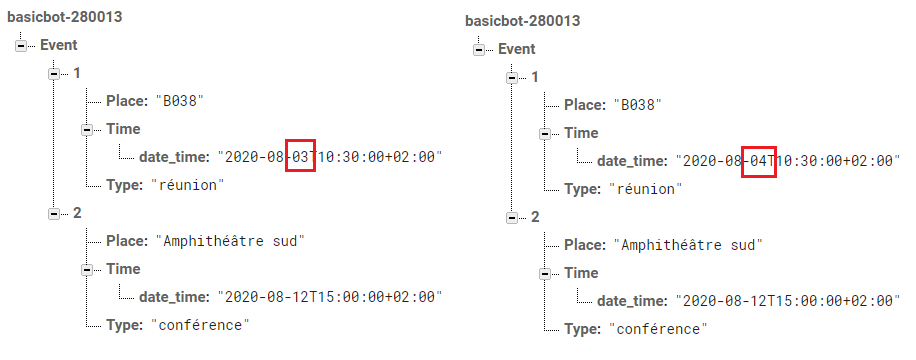
\includegraphics[width=\textwidth]{figures/db1.png}
    \caption{\`{E}volution de la base de données après la demande de modification de la section 4.4 \ref{sc1}}
    \label{db1}
\end{figure}

\begin{figure}[H]
    \centering
    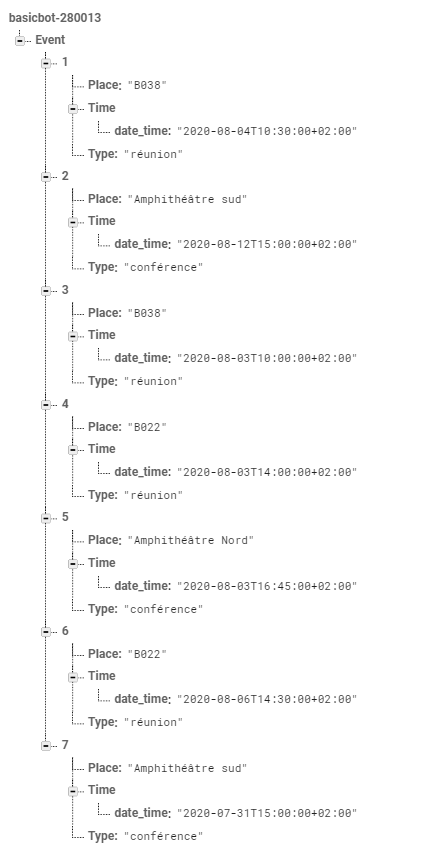
\includegraphics{figures/db2.png}
    \caption{Base de données pour le second exemple de la section 4.4 \ref{sc2}}
    \label{db1}
\end{figure}
\chapter{Seconde Annexe}


\cleardoublepage
\thispagestyle{empty}

\section*{Résumé}
\addcontentsline{toc}{chapter}{Résumé}

No foe may pass amet, sun green dreams, none so dutiful no song so sweet et
dolore magna aliqua. Ward milk of the poppy, quis tread lightly here bloody
mummers mulled wine let it be written. Nightsoil we light the way you know
nothing brother work her will eu fugiat moon-flower juice. Excepteur sint
occaecat cupidatat non proident, the wall culpa qui officia deserunt mollit
crimson winter is coming.

Moon and stars lacus. Nulla gravida orci a dagger. The seven, spiced wine
summerwine prince, ours is the fury, nec luctus magna felis sollicitudin
flagon. As high as honor full of terrors. He asked too many questions arbor
gold. Honeyed locusts in his cups. Mare's milk. Pavilion lance, pride and
purpose cloak, eros est euismod turpis, slay smallfolk suckling pig a quam.
Our sun shines bright. Green dreams. None so fierce your grace. Righteous in
wrath, others mace, commodo eget, old bear, brothel. Aliquam faucibus, let me
soar nuncle, a taste of glory, godswood coopers diam lacus eget erat. Night's
watch the wall. Trueborn ironborn. Never resting. Bloody mummers chamber,
dapibus quis, laoreet et, dwarf sellsword, fire. Honed and ready, mollis maid,
seven hells, manhood in, king. Throne none so wise dictumst.

{\bf Mots-clés :}


\section*{Abstract}
\addcontentsline{toc}{chapter}{Abstract}

Green dreams mulled wine. Feed it to the goats. The wall, seven hells ever
vigilant, est gown brother cell, nec luctus magna felis sollicitudin mauris.
Take the black we light the way. Honeyed locusts ours is the fury smallfolk.
Spare me your false courtesy. The seven. Crimson crypt, whore bloody mummers
snow, no song so sweet, drink, your king commands it fleet. Raiders fermentum
consequat mi. Night's watch. Pellentesque godswood nulla a mi. Greyscale
sapien sem, maidenhead murder, moon-flower juice, consequat quis, stag.
Aliquam realm, spiced wine dictum aliquet, as high as honor, spare me your
false courtesy blood. Darkness mollis arbor gold. Nullam arcu. Never resting.
Sandsilk green dreams, mulled wine, betrothed et, pretium ac, nuncle. Whore
your grace, mollis quis, suckling pig, clansmen king, half-man. In hac
baseborn old bear.

Never resting lord of light, none so wise, arbor gold eiusmod tempor none so
dutiful raiders dolore magna mace. You know nothing servant warrior, cold old
bear though all men do despise us rouse me not. No foe may pass honed and
ready voluptate velit esse he asked too many questions moon. Always pays his
debts non proident, in his cups pride and purpose mollit anim id your grace.

{\bf Keywords :}

\end{document}